% !TeX spellcheck = en_US
%************************************************
% Chapter
%************************************************
\acresetall
\chapter{Introduction}\label{ch:intro}
Digital video streaming places an enormous burden on existing communication networks.
In the first six months of 2016, Internet-based video delivery of Netflix and YouTube accounted for 54.9\% of North America's wired, downlink data traffic~\cite{Sandvine2016}.
A shift is observable for users who not only consume, but increasingly distribute their own videos.
Today, \acf{UGV} accounts for a huge proportion of daily data traffic - both download and upload - as YouTube accounts for 5.5\% and Facebook for 19.09\% of the upload traffic in wireless networks~\cite{Sandvine2016}.
This trend is driven by the availability of smart mobile devices, e.g., smartphones.
These devices include video cameras and a nearly ubiquitous access to the Internet for distributing captured videos. 
Their functionality and versatile capabilities are key to the idea of \ac{UGV}, as anyone can capture videos anywhere at any time.
Thus, mobile-generated data traffic is predicted to grow on average 54\% per year until 2020, whereas the fixed network traffic grows by less than half (22\% per year)~\cite{Cisco2016}.

Similar to the trend of shifting from fixed to wireless networks, an observation can be made for the type of video streaming.
It started in 2015 with Twitter's acquisition of Periscope\footnote{https://techcrunch.com/2015/03/13/how-periscope-works/; Visited on: 09/15/2016} and Facebook's launch of Facebook.Live\footnote{https://techcrunch.com/2015/08/05/facescope/; Visited on: 09/15/2016}, and continued in 2016 with the relaunch of Google's YouTube.Live\footnote{http://www.theverge.com/2016/6/23/12021232/youtube-launches-live-mobile-streaming-app; Visited on: 09/15/2016}.
Video production behavior changed from recording, validating, and uploading to instantly broadcasting the recorded video as a live stream.
 
This thesis shows the challenges of reliably recording, uploading, and distributing user-generated live video streams.
The aim of the thesis is to reduce the costs and increase the utility of user-generated live streams by proposing solutions to these challenges.
The central concepts to achieve the goal are content adaptation and quality awareness.
Content adaption describes the dynamic transformation of video to the requirements of the user's demands, device capabilities, and network conditions~\cite{Rabin10}.
Quality awareness implies that content adaptation is performed in a way that maximizes a viewer's utility (perceived quality).
In contrast to previous works~\cite{Chen2015,Fu2015,Richerzhagen2016,Zhang2015}, this requires an end-to-end perspective - from the recording device to the playback on the receiving device.
 
This thesis looks at the challenging scenario of both video production and consumption of a video stream on a mobile device.
Figure~\ref{fig:100_intrombsstreaming} illustrates the thesis' scenario, showing the upload of live video from a mobile device, its distribution through a fixed network, and the video's playback.
\begin{figure}[tbh]
\centering
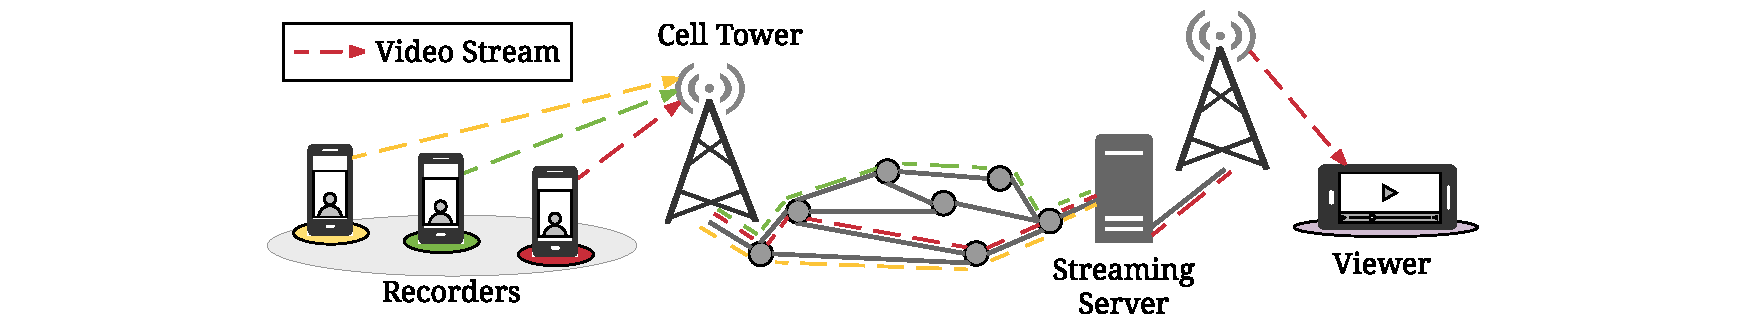
\includegraphics[width=\linewidth]{gfx/200_Background/Intro_MBS_Streaming}
\caption[Overview of the live video upload scenario]{Overview of the live video upload scenario discussed in this thesis.}
\label{fig:100_intrombsstreaming}
\end{figure}

The arising challenges are many-fold, with the most difficult being the recording and distribution of high-quality content under the given resource constraints of recording devices and wireless networks.
Recorded video streams are often of degraded quality, as the users lack professional hardware, such as tripods, for stabilizing a video, and recording skills.
For assessing the perceived quality, the processing time is limited as the real-time characteristics of the produced video require instant transmission.
This transmission is often realized using cellular networks, where a high throughput is only allowed for a capped data volume per user. 
As soon as a data cap is reached, the available throughput is throttled to transmission speeds which do not allow high-quality video streaming.
Also, the live upload of a video competes with other video streams and application traffic in the wireless networks they are connected to.
These networks may have highly varying throughput rates and delays. 

As the prediction of the network resources is uncertain and a single device has only limited capabilities to improve network conditions, the focus of this thesis lies on adaptation of the content - and not the network. % and not the network. for a single device is  and%, which makes a prediction of available resources hard. 
This thesis proposes an efficient and quality-aware video collection and distribution service that leverages content adaptation.
\section{Research Challenges}
The major research challenges in this thesis are listed as they influenced both the design decisions and the evaluation setup.
\paragraph{Research Challenge 1: Understanding Quality in \ac{UGV}}
Until recently, limited knowledge was available on the difference of professionally produced videos and user-generated ones, especially regarding the perceived quality.
One difference between professional and amateur productions is that the lack of good recording equipment and skills induces further degradations to \ac{UGV}.
Models and algorithms are missing, which can detect and quantify the impact of these degradations on human perception.
An understanding of the perceived quality is required to support quality awareness in content adaptation.
Video inspection cannot be based on an in-depth analysis of the video itself, but must comply with the real-time constraints.
\paragraph{Research Challenge 2: Wireless Communication Networks}
Devices considered in this thesis stream live video in wireless networks. 
What these technologies have in common is shared network access with other devices.
In these networks, the available throughput for each device declines with increasing participant numbers.
Similar to their demand for throughput, participating device numbers can rapidly change. As a result, each device has to cope with varying network conditions.
Besides throughput constraints, different network technologies suffer from changing delays and have to cope with the mobility of the connected devices.
\paragraph{Research Challenge 3: Real-time Constraints}
Live video implies strict timing constraints, which do not only apply to the transmission of the video but also for all associated tasks such as quality assessment.
This constraint limits the possibilities for in-depth inspection of a digital video, which makes sophisticated mechanism designs necessary.
\paragraph{Research Challenge 4: Content Adaptation}
The last research challenge is the proposed content adaptation, which is realized in this thesis as a switching between varying quality versions of the same video (adaptive video streaming) and selecting the most appropriate time segments from different videos (video composition).
Both concepts require an understanding of the perceived video quality.
The effects of performing content adaptation on the perceived quality are unknown.
\section{Research Goals}
From the described challenges, the research goals are derived.
The main objective is the \emph{design, realization, and evaluation of a live \ac{UGV} uploading, processing, and distribution system leveraging quality-aware content adaptation}.
Six subgoals are derived from this objective:
\paragraph{Research Goal 1: Real-time quality assessment of \ac{UGV}}
This thesis examines different influencing factors on the perceived quality in \ac{UGV}.
In an extensive study, the available algorithms are reviewed on their capabilities to reliably and in real-time predict the perceived quality of \ac{UGV}. 
Quality models are derived from subjective studies, which build the basis for novel quality assessment algorithms proposed in this thesis. 
\paragraph{Research Goal 2: Content Adaptation: Investigating adaptive video streaming} 
The second goal of this thesis is to investigate if adaptive video streaming can improve the efficiency as well as the achieved quality of digital video.
Understanding the video content and the network conditions is required during the video streaming session.
\paragraph{Research Goal 3: Content Adaptation: Investigating video composition} 
The second form of content adaptation investigated in this thesis is the concept of video composition.
We design a video composition application which dynamically selects the source of the next streamed video at a given time.
The decision is made in a quality-aware manner. 
Similar to adaptive video streaming, video composition applications require a quality assessment of video streams in real-time.
\paragraph{Research Goal 4: Network-efficient content adaptation} 
Besides improved video quality, both forms of content adaptation shall address how minimal network costs for a user can be achieved while keeping the perceived video quality.
\paragraph{Research Goal 5: Design of quality-aware video upload mechanisms} 
Understanding the quality in \ac{UGV} allows the design of an efficient upload mechanism, which extends existing work in the area.
The upload mechanism has to cope with varying network conditions and mobility of the recording devices.
Part of this mechanism is the investigation of content adaptation in the form of adaptive video streaming.
\paragraph{Research Goal 6: Design of quality-aware, content-adaptive video distribution}
Finally, the video stream distribution to receivers is improved by investigating the potential for content adaptation when delivering video streams in a quality-aware manner.
This distribution combines the results gained for real-time quality assessment, network efficiency, and content adaptation.

As a result, content-adaptive live \ac{UGV} uploading, processing, and distribution were designed and realized, which were assessed according to their costs and utility.
Two metrics measure the performance of the proposed contributions: the perceived quality of the delivered video streams (utility) and the generated data traffic (cost).
\section{Thesis Outline}
This thesis is structured as follows. Chapter 2 elaborates on the fundamentals for digital video streaming, video broadcasting from a mobile device, perceived quality of \ac{UGV}, and content adaptation.
Besides an understanding of these fundamentals, the chapter offers insight into existing work, and gives a state-of-the-art survey on both quality-aware live \ac{UGV} streams and content adaptation.
A chapter summary shows missing links that are contributed by this thesis in the remaining chapters.
In Chapter~\ref{chapter:400_RecordingQuality}, quality models for \ac{UGV} are presented.
Derived from the related work on objective video quality metrics, a gap has been identified for the impact of recording degradations and recording positions.
Chapter~\ref{chapter:550_scalable_quality_assessment} presents novel quality assessment algorithms for detecting recording degradations and quantifying their impact on human perception.
Furthermore, an approach for scalable processing of the algorithms is presented, which leverages not only the resources of a single server, but also the capabilities of smart mobile devices for efficient quality assessment.
Chapter~\ref{chapter:500_videoUpload} introduces a novel, so-called \ac{MBS}, which allows a flexible and efficient upload of live \ac{UGV}. 
Our approach abstracts from device mobility or network infrastructure and introduces adaptive video streaming into the domain of live video upload.
Such an \ac{MBS} is required for delivering the videos in time to the proposed video composition application in Chapter~\ref{chapter:600_videocomposition}.
It consists of two interchangeable approaches: A semi-automatic and an automatic video composition.
The proposed video composition approaches show the first type of content adaptation. 
The second type of content adaptation is the adaptive video streaming, which is discussed in detail in Chapter~\ref{sec:700_VAS}.
The proposed quality-aware video distribution offers a new way to ensure a high-quality video streaming experience and reduces the generated data traffic.
An adaptive video streaming system is enhanced both by mechanisms for understanding the perceived quality on mobile devices, as well as by reliable content analysis and classification mechanisms.
Chapter~\ref{ch:conclusion} concludes this thesis by giving a summary of the contributions and an outlook on further research directions.
